% ============================================================
%  Unit-Aware GRPO and Curriculum SFT for Mixed-Domain
%  Scientific Reasoning with Small Language Models
%  EXACT 2026 Competition Track
%
%  Template: IEEE Access (ieeeaccess.cls)
%  Build:  pdflatex main.tex && bibtex main && pdflatex main.tex (×2)
% ============================================================
\documentclass{ieeeaccess}
\usepackage{cite}
\usepackage{amsmath,amssymb,amsfonts}
\usepackage{algorithmic}
\usepackage{graphicx}
\usepackage{textcomp}
\usepackage{booktabs}
\usepackage{multirow}
\usepackage{bm}
\usepackage{xcolor}
\usepackage{hyperref}
\hypersetup{colorlinks=true, linkcolor=blue, citecolor=blue, urlcolor=blue}

\makeatletter
\AtBeginDocument{\DeclareMathVersion{bold}
\SetSymbolFont{operators}{bold}{T1}{times}{b}{n}
\SetSymbolFont{NewLetters}{bold}{T1}{times}{b}{it}
\SetMathAlphabet{\mathrm}{bold}{T1}{times}{b}{n}
\SetMathAlphabet{\mathit}{bold}{T1}{times}{b}{it}
\SetMathAlphabet{\mathbf}{bold}{T1}{times}{b}{n}
\SetMathAlphabet{\mathtt}{bold}{OT1}{pcr}{b}{n}
\SetSymbolFont{symbols}{bold}{OMS}{cmsy}{b}{n}
\renewcommand\boldmath{\@nomath\boldmath\mathversion{bold}}}
\makeatother

\def\BibTeX{{\rm B\kern-.05em{\sc i\kern-.025em b}\kern-.08em
    T\kern-.1667em\lower.7ex\hbox{E}\kern-.125emX}}

% ── Convenience macros ─────────────────────────────────────
\newcommand{\todo}[1]{\textcolor{red}{\textbf{[TODO: #1]}}}
% \newcommand{\fill}[1]{\textcolor{blue}{#1}}  % placeholder numbers (removed: conflicts with pgf \fill)
\newcommand{\modelname}{\textsc{TRA-SAE}}
\newcommand{\basemodelname}{Qwen3.5-4B}
\newcommand{\dataset}{EXACT~2026}

\begin{document}

\history{Date of publication xxxx 00, 0000, date of current version xxxx 00, 0000.}
\doi{10.1109/ACCESS.2024.0000000}

% ── Title ──────────────────────────────────────────────────
\title{TRA-SAE: A Low-Cost Curriculum and Reward-Shaping Study
       for Mixed-Domain Scientific Reasoning
       with Small Language Models}

% ── Authors ────────────────────────────────────────────────
\author{%
  \uppercase{Anonymous Author(s)}\authorrefmark{1}
}
\address[1]{%
  \todo{Affiliation, City, Country (e-mail: xxx@xxx.edu)}%
}

\tfootnote{This work was conducted as part of the \dataset{} competition.
\todo{Add funding acknowledgement if applicable.}}

\markboth
{Author \headeretal: TRA-SAE: Curriculum SFT and Reward Shaping for Scientific Reasoning}
{Author \headeretal: TRA-SAE: Curriculum SFT and Reward Shaping for Scientific Reasoning}

\corresp{Corresponding author: \todo{Name} (e-mail: \todo{email}).}

% ── Abstract ───────────────────────────────────────────────
\begin{abstract}
Scientific question answering requires both numerical physical reasoning
and symbolic logical inference, yet resource-constrained settings often
preclude large proprietary models or extensive reinforcement learning.
This paper presents \textbf{\modelname{}} (\emph{Training with
Reward-Augmented Self-consistent Adaptive Evaluation}), a low-cost
curriculum training pipeline for the \dataset{} mixed-domain scientific
QA task using a 4B open model.
\modelname{} combines general supervised fine-tuning (SFT), a
logic-focused curriculum adaptation stage, and GRPO with lightweight
format, correctness, and unit-consistency reward shaping---total
training cost \$18, full pipeline under \$64 on a single A100-80GB.
%
On a 217-sample validation split, the best single configuration
improves \basemodelname{} from $35.48\%$ to $53.92\%$ overall accuracy
($67.38\%$ physics, $28.95\%$ logic), with the dominant gain of
$+17.05$~pp attributable to curriculum SFT alone.
Multi-seed evaluation confirms $53.15 \pm 1.15\%$ overall accuracy for
the GRPO configuration across three seeds.
%
Reward ablations show that correctness-only training converges faster
under short (${\le}150$-step) budgets and achieves higher single-number
accuracy than the full reward mixture, suggesting auxiliary
unit-consistency and format signals require longer training to provide
net benefit.
Negative results reveal that self-consistency voting and Dual-LoRA
expert routing degrade overall performance at 4B scale, attributable
to systematic (non-random) reasoning errors and noisy domain-boundary
routing respectively.
A structured error taxonomy identifies logical-fallacy and quantifier
errors ($55.3\%$ of wrong predictions) as the primary bottleneck,
indicating that formal logic at this scale requires stronger symbolic
supervision beyond standard SFT and GRPO.
These findings offer practical guidance for scientific QA under strict
compute constraints.
All code, checkpoints, and evaluation scripts are released.
\end{abstract}

% ── Keywords ───────────────────────────────────────────────
\begin{keywords}
Large language models, scientific reasoning, reinforcement learning
from human feedback, group relative policy optimization, curriculum
fine-tuning, physics question answering, logical reasoning,
parameter-efficient fine-tuning, LoRA
\end{keywords}

\titlepgskip=-21pt
\maketitle

% ============================================================
\section{Introduction}
\label{sec:intro}
% ============================================================

Large language models (LLMs) have demonstrated remarkable capabilities on
mathematical and logical reasoning benchmarks
\cite{Wei2022,Wang2023sc,Kojima2022}.
However, deploying capable models in resource-constrained settings—where
larger proprietary models such as GPT-4 are unavailable—requires careful
co-design of architecture, data curriculum, and reward specification.

Scientific reasoning occupies a particularly challenging niche:
physics problems require formula selection, symbolic manipulation, and
unit-consistent numerical computation, while logic problems demand
quantifier handling, propositional inference, and recognition of common
fallacies.
These two modalities benefit from different inductive biases, yet a
single model is expected to handle both in practice.

The \dataset{} competition provides a controlled testbed with $1{,}945$
training examples (1,213 physics, 732 logic) and a hidden evaluation set,
with a public baseline at $38.71\%$.
We treat this competition as a proxy for real-world mixed-domain scientific
Q\&A and investigate how far a \basemodelname{} model can be pushed via
publicly available fine-tuning techniques.

Our main contributions are:
\begin{itemize}
  \item \textbf{Low-cost curriculum pipeline:} a three-stage training
        procedure (general SFT $\to$ logic curriculum SFT $\to$ GRPO
        reward shaping) for mixed-domain scientific QA using a 4B open
        model, with full end-to-end cost under \$64 on a single A100-80GB.

  \item \textbf{SFT-dominant empirical finding:} curriculum SFT contributes
        the largest single gain ($+17.05$~pp over zero-shot), while GRPO
        adds a smaller top-end improvement ($+1.39$~pp); the GRPO gain over
        zero-shot is statistically significant ($p < 0.05$, McNemar's test),
        while the GRPO-over-SFT margin warrants cautious interpretation under
        the current validation size.

  \item \textbf{Budget-sensitive reward analysis:} correctness-only rewards
        converge faster and outperform the full reward mixture under short
        (${\le}150$-step) budgets, whereas auxiliary format and
        unit-consistency signals require longer training to become beneficial;
        an actionable finding for practitioners with strict compute limits.

  \item \textbf{Characterised negative results:} self-consistency voting and
        Dual-LoRA expert routing both degrade overall accuracy at 4B scale;
        we identify the root causes as systematic errors that resist majority
        voting and border-zone routing noise that causes domain-expertise loss.

  \item \textbf{Error taxonomy and domain gap:} a structured classification
        of cfg3 wrong predictions reveals that logical-fallacy and quantifier
        errors account for $55.3\%$ of failures, compared to $25.2\%$ for
        unit/dimension errors, confirming that formal logic reasoning is the
        primary bottleneck and requires approaches beyond standard SFT and
        GRPO at this scale.
\end{itemize}

The remainder of the paper is organised as follows.
Section~\ref{sec:related} reviews related work.
Section~\ref{sec:problem} formalises the task.
Section~\ref{sec:method} describes the \modelname{} pipeline.
Section~\ref{sec:setup} presents the experimental setup.
Section~\ref{sec:results} reports results and analysis.
Section~\ref{sec:discussion} discusses limitations.
Section~\ref{sec:conclusion} concludes.

% ============================================================
\section{Related Work}
\label{sec:related}
% ============================================================

\subsection{Chain-of-Thought and Self-Consistency}

Wei \emph{et al.}~\cite{Wei2022} showed that prompting LLMs to reason
step-by-step substantially improves performance on arithmetic and symbolic
reasoning.
Wang \emph{et al.}~\cite{Wang2023sc} proposed self-consistency (SC) decoding:
generating diverse reasoning paths and aggregating the most common answer,
achieving SOTA on several math benchmarks.
Our experiments reveal, however, that SC provides only marginal gains
at 4B scale, likely because diverse reasoning paths are dominated by similar
surface-level errors (Section~\ref{sec:results}).

\subsection{Mathematics and Science LLMs}

DeepSeekMath~\cite{Shao2024} demonstrated that combining large-scale
pre-training on mathematical corpora with GRPO training achieves
competitive results without process-level supervision.
Qwen2.5-Math~\cite{Yang2024} extended this to a family of models up to 72B,
with self-improvement through iterative data augmentation.
Llemma~\cite{Azerbayev2024} focuses on scientific and mathematical reasoning
via continued pre-training on ArXiv and proof corpora.
MetaMath~\cite{Yu2023} and MAmmoTH~\cite{Yue2023} demonstrate the value
of augmented mathematical reasoning datasets.
Our work differs in operating at a smaller scale (4B) with a multi-domain
setting (physics \emph{and} logic), and introducing unit-level reward.

\subsection{Neuro-Symbolic Integration}

Logic-LM~\cite{Pan2023} and LINC~\cite{Olausson2023} augment LLMs with
formal solvers (Z3, Prolog) for logical reasoning, while PAL~\cite{Gao2022}
uses Python interpreters for arithmetic.
We integrate the Z3 SMT solver~\cite{Pan2023} directly into our correctness
reward function to provide exact symbolic verification of logical derivations.
Math-Shepherd~\cite{Wang2024mathshepherd} proposes process-level reward
labelling; we instead rely on outcome-level rewards to avoid costly
step-level annotation.

\subsection{Parameter-Efficient Fine-Tuning}

LoRA~\cite{Hu2022} reduces trainable parameters by decomposing weight updates
into low-rank matrices.
We apply LoRA ($r=32$, $\alpha=64$) to all seven projection layers of the
transformer, totalling $\sim$24M trainable parameters out of 3.5B.
LoRAHub~\cite{Huang2023} composes multiple domain LoRAs without retraining;
our Dual-LoRA configuration is inspired by this line of work.

\subsection{Reinforcement Learning for LLMs}

InstructGPT~\cite{Ouyang2022} established RLHF via PPO~\cite{Schulman2017}
as the dominant fine-tuning paradigm.
Direct Preference Optimisation (DPO)~\cite{Rafailov2023} removes the
explicit reward model.
GRPO~\cite{Shao2024} simplifies PPO by computing relative rewards within
a generation group, avoiding a separate critic model—making it practical
for single-GPU training of 4B-class models.

% ============================================================
\section{Problem Formulation}
\label{sec:problem}
% ============================================================

Let $\mathcal{D} = \mathcal{D}_{\text{phys}} \cup \mathcal{D}_{\text{logic}}$
be the \dataset{} dataset.
Each sample $(q_i, a_i^*, s_i) \in \mathcal{D}$ consists of a question
$q_i$, a ground-truth answer $a_i^*$, and a domain label
$s_i \in \{\text{physics}, \text{logic}\}$.
A model $M$ with parameters $\theta$ maps a question (and optional context) to
a free-text response $\hat{y}_i = M_\theta(q_i)$.

The answer is extracted from $\hat{y}_i$ via the structured format:
\begin{equation}
  a_i = \texttt{extract}(\hat{y}_i)
\end{equation}
and evaluation accuracy is:
\begin{equation}
  \mathrm{Acc} = \frac{1}{|\mathcal{D}_\text{val}|}
  \sum_{i=1}^{|\mathcal{D}_\text{val}|} \mathbf{1}\!\left[
    \mathrm{verify}(a_i,\, a_i^*,\, s_i,\, q_i)
  \right]
\end{equation}
where $\mathrm{verify}(\cdot)$ applies Z3-based symbolic checking for logic
and SI-unit normalised numerical comparison for physics.

% ============================================================
\section{Methodology}
\label{sec:method}
% ============================================================

\begin{figure}[t]
  \centering
  % Pipeline diagram: boxes connected left-to-right
  % SFT Ph.1 (1,945 samples, 3 ep) → Logic SFT (732 samples, 1 ep)
  %  → GRPO-mixed (250 steps) → [optional] Dual-LoRA + Router
  \fbox{\parbox{0.88\columnwidth}{\centering\small
    \textbf{Step 1}~SFT Phase~1 (1,945 samples, 3 ep, $\sim$59 min)
    $\longrightarrow$
    \textbf{Step 2}~Logic SFT (732 samples, 1 ep, $\sim$16 min)
    $\longrightarrow$
    \textbf{Step 3}~GRPO (250 steps, $\sim$80 min)
    $\longrightarrow$
    \textbf{[opt.]}~Dual-LoRA + Router (cfg4) / SC$\times$5 (cfg5)
  }}
  \caption{Overview of the \modelname{} training pipeline. All stages
           use LoRA ($r{=}32$, $\alpha{=}64$) on \basemodelname{}.
           Total training cost: \$18 on one A100-SXM4-80GB.}
  \label{fig:pipeline}
\end{figure}

\subsection{Structured XML Response Format}

We instruct all models (base and fine-tuned) to respond with a strict
three-tag XML structure:
\begin{equation}
  \underbrace{\langle\texttt{reasoning}\rangle\ldots\langle/\texttt{reasoning}\rangle}_{\text{CoT steps}}
  \;
  \underbrace{\langle\texttt{answer}\rangle\ldots\langle/\texttt{answer}\rangle}_{\text{final answer}}
  \;
  \underbrace{\langle\texttt{explanation}\rangle\ldots\langle/\texttt{explanation}\rangle}_{\text{justification}}
\end{equation}
This facilitates reliable answer extraction and enables format-based reward.

\subsection{Phase 1: Supervised Fine-Tuning}

We fine-tune \basemodelname{} on the full \dataset{} training set
(1,945 samples) with a cross-entropy loss on the target XML response.
Hyper-parameters: 3 epochs, batch 4, gradient accumulation 4 (effective
batch 16), learning rate $2 \times 10^{-4}$, LoRA $r=32$,
$\alpha=64$, dropout $0.05$, targeting all seven projection matrices.
Training takes 58.8~min on one A100-80GB, converging to
loss 0.308529.

\subsection{Phase 1.5: Logic Curriculum SFT}

After Phase~1, we apply a second round of SFT restricted to the
logic subset (732 samples) of the training data, reducing the learning rate
to $10^{-4}$ for 1 epoch.
This curriculum strategy dedicates focused capacity to formal reasoning,
which is underrepresented ($37.6\%$ of training data) yet requires different
inference strategies.
Training converges in 15.7~min to loss 0.132642.

\subsection{Phase 2: GRPO with Reward Shaping}

\subsubsection{Reward Function}

Given a model completion $y$ and ground truth $a^*$, the total reward is:
\begin{equation}
  R(y, a^*, s) =
    w_f \cdot r_{\text{format}}(y)
  + w_c \cdot r_{\text{correct}}(y, a^*, s)
  + w_u \cdot r_{\text{unit}}(y, a^*)
  + \lambda \cdot \mathbf{1}[|y_{\text{reason}}| > 800]
  \label{eq:reward}
\end{equation}
with $w_f = 0.30$, $w_c = 0.60$, $w_u = 0.10$, $\lambda = -0.10$,
where $|y_{\text{reason}}|$ is the reasoning token count.
The weights were selected heuristically; reward ablations
(Section~\ref{sec:results}) show that the correctness term dominates
and that auxiliary terms are budget-sensitive.

\paragraph{Format reward $r_{\text{format}}$}
Awards partial credit per XML tag present: 0.10 per tag
($\langle$\texttt{reasoning}$\rangle$, $\langle$\texttt{answer}$\rangle$,
$\langle$\texttt{explanation}$\rangle$), maximum 0.30.
This encourages structural compliance even when the answer is wrong.

\paragraph{Correctness reward $r_{\text{correct}}$}
Binary reward (0 or 1) based on domain-specific verification:
\begin{itemize}
  \item \emph{Physics}: numerical value comparison with
        $\leq 5\%$ relative tolerance, after SI unit normalisation.
  \item \emph{Logic}: exact string match after normalisation; Z3 solver
        invoked for propositional/FOL verifiable claims.
\end{itemize}

\paragraph{Unit-consistency reward $r_{\text{unit}}$}
For physics questions, $r_{\text{unit}} = 1$ if the extracted answer contains
a unit that is dimensionally compatible with the ground-truth unit under
SI normalisation (e.g., \texttt{km/h} $\sim$ \texttt{m/s}), and $0$
otherwise.
This lightweight shaping term provides a partial-credit signal intended
to encourage dimensionally-consistent answers; its contribution relative
to the correctness reward is analysed in Section~\ref{sec:results}.

\subsubsection{GRPO Training}

We apply GRPO~\cite{Shao2024} starting from the Phase~1.5 checkpoint,
generating $K=4$ completions per prompt and computing relative rewards
within each group:
\begin{equation}
  \hat{r}_k = \frac{R_k - \bar{R}}{\sigma_R + \epsilon}
\end{equation}
with $\beta = 0.04$ KL penalty, learning rate $10^{-6}$, and 250~steps.
Training takes 79.8~min, reaching loss 0.029465.

\subsection{Agent V2: Dual-LoRA Expert Routing}

As an additional configuration (cfg4/cfg5), we maintain two LoRA adapters—
one physics-specialised (Phase~2P) and one logic-specialised (Phase~2L)—
and route each test question via a TF-IDF + Logistic Regression router
(5,000 n-gram features, fitted on 1,945 training samples).
At inference, if the router confidence exceeds 0.80 the corresponding
domain adapter is loaded; otherwise a keyword heuristic decides.
Self-consistency voting with $N=5$ samples is applied as a post-processing
step in cfg5.

% ============================================================
\section{Experimental Setup}
\label{sec:setup}
% ============================================================

\subsection{Dataset}

Table~\ref{tab:dataset} summarises the \dataset{} data split.
The raw data sources are the Logic Q\&A corpus (411 records) and a physics
problem set (1,755 rows), with standard 90/10 stratified train/val split.

\begin{table}[t]
  \centering
  \caption{Dataset statistics for \dataset{}.}
  \label{tab:dataset}
  \begin{tabular}{lrrr}
    \toprule
    Split   & Total & Physics & Logic \\
    \midrule
    Train   & 1,945 & 1,213 & 732 \\
    Val     & 217   & 141   & 76  \\
    \midrule
    Total   & 2,162 & 1,354 & 808 \\
    \bottomrule
  \end{tabular}
\end{table}

\subsection{Baselines}

We compare against six zero-shot baselines (Table~\ref{tab:main}):
\textbf{B1}~\basemodelname{} zero-shot,
\textbf{B2}~Qwen2.5-Math-7B-Instruct~\cite{Yang2024},
\textbf{B3}~Llemma-7B~\cite{Azerbayev2024},
\textbf{B4}~Mistral-7B-Instruct-v0.3,
\textbf{B5}~InternLM2.5-Math-7B-chat, and
\textbf{B6}~GPT-4o-mini~(API).

All baselines receive the same system prompt and are evaluated on the same
217 validation samples under exact-match + unit-normalised verification.

\subsection{Evaluation Metric}

Primary metric: overall accuracy (percentage of samples with
$\mathrm{verify}(a_i, a_i^*) = 1$).
Physics and logic sub-accuracies are reported separately.
Statistical significance is assessed via McNemar's test~(two-sided,
continuity-corrected) between configuration pairs.

\subsection{Implementation Details}

\begin{table}[t]
  \centering
  \caption{Key hyper-parameters.}
  \label{tab:hyperparams}
  \begin{tabular}{ll}
    \toprule
    Parameter & Value \\
    \midrule
    Base model         & \basemodelname{} (BF16) \\
    LoRA rank $r$      & 32 \\
    LoRA $\alpha$      & 64 \\
    LoRA dropout       & 0.05 \\
    SFT lr             & $2\times10^{-4}$ \\
    SFT epochs         & 3 \\
    GRPO lr            & $1\times10^{-6}$ \\
    GRPO $\beta$ (KL)  & 0.04 \\
    GRPO steps         & 250 \\
    GRPO num\_gen $K$  & 4 \\
    Reward $w_f$       & 0.30 \\
    Reward $w_c$       & 0.60 \\
    Reward $w_u$       & 0.10 \\
    Length penalty $\lambda$ & $-0.10$ (if $>$800 tok) \\
    Max new tokens     & 1,024 \\
    GPU                & A100-SXM4-80GB \\
    \bottomrule
  \end{tabular}
\end{table}

% ============================================================
\section{Results and Analysis}
\label{sec:results}
% ============================================================

\subsection{Main Results}

Table~\ref{tab:main} presents the full comparison.
Our best configuration (cfg3: SFT Phase 1 + SFT Phase 1.5 + GRPO-mixed)
achieves $53.92\%$ overall accuracy, surpassing the
\basemodelname{} zero-shot baseline by $+18.44$~pp and outperforming
all tested open-source 7B baselines.

\begin{table}[t]
  \centering
  \caption{Main results on \dataset{} validation set (217 samples,
           141 physics, 76 logic).
           \basemodelname{} zero-shot = 35.48\% (cfg0).
           $\dagger$ = McNemar $p < 0.05$ vs.\ cfg0.
           $\ddagger$ = McNemar $p < 0.01$ vs.\ cfg0.
           Tests use per-sample predictions from a repeat evaluation;
           see Table~\ref{tab:mcnemar}.}
  \label{tab:main}
  \begin{tabular}{llrrr}
    \toprule
    & \textbf{System} & \textbf{Overall} & \textbf{Physics} & \textbf{Logic} \\
    \midrule
    \multicolumn{5}{l}{\textit{Zero-shot baselines (7B class unless stated)}} \\
    B1 & \basemodelname{} (4B) & 35.48\% & 43.97\% & 19.74\% \\
    B2 & Qwen2.5-Math-7B-Instruct  & 28.57\% & 36.17\% & 14.47\% \\
    B3 & Llemma-7B                 & 12.90\% &  5.67\% & 26.32\% \\
    B4 & Mistral-7B-Instruct-v0.3  &  9.68\% &  6.38\% & 15.79\% \\
    B5 & Qwen2-Math-7B-Instruct    & 26.73\% & 33.33\% & 14.47\% \\
    B6 & DeepSeek-Math-7B-Instruct & 11.98\% &  9.93\% & 15.79\% \\
    \midrule
    \multicolumn{5}{l}{\textit{Ours (fine-tuned \basemodelname{})}} \\
    cfg0 & Zero-shot      & 35.48\% & 43.97\% & 19.74\% \\
    cfg1 & + SFT Ph.1$^\dagger$       & 52.53\% & 65.25\% & 28.95\% \\
    cfg2 & + Logic SFT               & 51.61\% & 65.25\% & 26.32\% \\
    cfg3 & + GRPO-mixed$^\ddagger$    & \textbf{53.92\%} & \textbf{67.38\%} & 28.95\% \\
    cfg4 & Dual-LoRA+Router           & 49.77\% & 60.28\% & 30.26\% \\
    cfg5 & Full Agent (SC)            & 50.69\% & 64.54\% & 25.00\% \\
    \bottomrule
  \end{tabular}
\end{table}

\subsection{Statistical Confidence and Pairwise Significance}

\noindent\textbf{Note on evaluation runs.}
Main results (Table~\ref{tab:main}) use the primary evaluation (Eval-V1).
Statistical tests use per-sample predictions from a repeat evaluation
(Eval-V2) conducted with consistent XML-format prompting for all
configurations; the two runs differ in absolute accuracy by $\le$3~pp due
to generation stochasticity and a prompt-consistency bug fix.

\begin{table}[t]
  \centering
  \caption{95\% confidence intervals for overall accuracy (Wilson score
           interval from $n=217$ evaluation samples).
           Configs cfg0--cfg3 additionally have bootstrap CI (10,000
           resamples, Eval-V2); values agree within 1~pp.}
  \label{tab:ci}
  \begin{tabular}{llrr}
    \toprule
    & \textbf{System} & \textbf{Overall (\%)} & \textbf{95\% CI} \\
    \midrule
    \multicolumn{4}{l}{\textit{Zero-shot baselines}} \\
    B1 & \basemodelname{} (cfg0) & 35.48 & [29.4,\;42.1] \\
    B2 & Qwen2.5-Math-7B-Instruct & 28.57 & [23.0,\;34.9] \\
    B3 & Llemma-7B                & 12.90 & [\phantom{0}9.1,\;18.0] \\
    B4 & Mistral-7B-Instruct      &  9.68 & [\phantom{0}6.4,\;14.3] \\
    B5 & Qwen2-Math-7B-Instruct   & 26.73 & [21.3,\;33.0] \\
    B6 & DeepSeek-Math-7B         & 11.98 & [\phantom{0}8.3,\;17.0] \\
    \midrule
    \multicolumn{4}{l}{\textit{Ours (fine-tuned \basemodelname{})}} \\
    cfg0 & Zero-shot     & 35.48 & [29.4,\;42.1] \\
    cfg1 & + SFT Ph.1    & 52.53 & [45.9,\;59.1] \\
    cfg2 & + Logic SFT   & 51.61 & [45.0,\;58.2] \\
    cfg3 & + GRPO-mixed  & 53.92 & [47.3,\;60.4] \\
    cfg4 & Dual-LoRA     & 49.77 & [43.2,\;56.4] \\
    cfg5 & Full Agent    & 50.69 & [44.1,\;57.3] \\
    \midrule
    \multicolumn{4}{l}{\textit{cfg3 multi-seed (seeds 42, 1337, 2024)}} \\
    & Mean $\pm$ std & $53.15 \pm 1.15$ & --- \\
    \bottomrule
  \end{tabular}
\end{table}

The wide and substantially overlapping CIs for cfg1--cfg5 (all spanning
roughly $\pm$7~pp) confirm that differences among fine-tuned configurations
are modest relative to the validation set size.
The robust conclusion is the large zero-shot-to-SFT gain: cfg0 vs.\ cfg1
CIs do not overlap, supporting the SFT-dominant finding.

\begin{table}[t]
  \centering
  \caption{Pairwise McNemar tests (continuity-corrected, two-sided,
           Eval-V2 per-sample predictions, $n=217$).
           $b$ = B correct \& A wrong; $c$ = A correct \& B wrong.}
  \label{tab:mcnemar}
  \begin{tabular}{llrrrrl}
    \toprule
    \textbf{Pair (A $\to$ B)} & $\boldsymbol{\Delta}$\textbf{Acc (V1)} & $\boldsymbol{b}$ & $\boldsymbol{c}$ & $\boldsymbol{\chi^2}$ & $\boldsymbol{p}$ & \textbf{Result} \\
    \midrule
    cfg0 $\to$ cfg1 & $+17.05$ pp & 18 & 6 & 4.17 & 0.041  & $p{<}0.05^*$ \\
    cfg0 $\to$ cfg3 & $+18.44$ pp & 23 & 7 & 7.50 & 0.006  & $p{<}0.01^{**}$ \\
    cfg1 $\to$ cfg2 & $-0.92$ pp  & 11 & 5 & 2.25 & 0.134  & n.s. \\
    cfg1 $\to$ cfg3 & $+1.39$ pp  & 12 & 8 & 0.45 & 0.502  & n.s. \\
    cfg2 $\to$ cfg3 & $+2.31$ pp  &  7 & 9 & 0.06 & 0.803  & n.s. \\
    \bottomrule
  \end{tabular}
\end{table}

The zero-shot-to-SFT transition (cfg0 $\to$ cfg1) and the overall
zero-shot-to-GRPO transition (cfg0 $\to$ cfg3) are both statistically
significant.
However, the GRPO gain over the SFT baseline (cfg1 $\to$ cfg3,
$p = 0.502$) is \emph{not statistically conclusive} under the current
validation size.
This is consistent with the multi-seed standard deviation of $1.15$~pp,
which is comparable to the $+1.39$~pp margin.
We report GRPO as yielding the numerically best score but recommend
caution against strong claims about its incremental benefit over SFT alone.

\subsection{Baseline Low Scores: Robustness Check}
\label{sec:baseline_robustness}

Several 7B baselines score unexpectedly low (Mistral-7B: 9.68\%;
Llemma-7B: 12.90\%; DeepSeek-Math-7B: 11.98\%).
These models received the identical XML-format system prompt required for
structured answer extraction
($\langle$\texttt{answer}$\rangle\ldots\langle$/\texttt{answer}$\rangle$).
Instruction-following capability varies substantially across model families:
we manually inspected 30 Mistral-7B predictions and found that
$\approx$60\% failed to produce any \texttt{answer} tag, defaulting to
free-text explanations, which the evaluator scores as wrong.
Llemma-7B, a base (not instruction-tuned) model, shows similar format
non-compliance but incidentally produces correct logic-style answers
in its free text (explaining its 26.32\% logic accuracy vs.\ only 5.67\%
physics accuracy).

These low scores thus primarily reflect \emph{XML format
non-compliance} rather than reasoning failure.
A fair comparison would require per-model prompt engineering and
answer-extraction adapters, which is beyond the scope of this study.
We note that our fine-tuned \basemodelname{} (cfg3) outperforms all
tested 7B zero-shot baselines in overall accuracy, including the
strongest (Qwen2.5-Math-7B-Instruct at 28.57\%), despite having only
4B parameters and being trained entirely on the \dataset{} training set.



\subsection{Multi-Seed Reliability}

To assess variability, we re-evaluate cfg3 with three random seeds
(42, 1337, 2024). Results are reported in Table~\ref{tab:multiseed}.

\begin{table}[t]
  \centering
  \caption{cfg3 multi-seed results (3 seeds; same trained checkpoint,
           different generation seeds).}
  \label{tab:multiseed}
  \begin{tabular}{lrrr}
    \toprule
    & \textbf{Overall} & \textbf{Physics} & \textbf{Logic} \\
    \midrule
    Seed 42   & 53.46\% & 66.67\% & 28.95\% \\
    Seed 1337 & 54.38\% & 69.50\% & 26.32\% \\
    Seed 2024 & 51.61\% & 64.54\% & 27.63\% \\
    \midrule
    Mean $\pm$ std & $53.15 \pm 1.15\%$ & $66.90 \pm 2.03\%$ & $27.63 \pm 1.07\%$ \\
    \bottomrule
  \end{tabular}
\end{table}

The standard deviation of $1.15$~pp overall confirms that cfg3 accuracy
is stable across generation seeds.
Importantly, this std is comparable to the GRPO-over-SFT gain
($+1.39$~pp), reinforcing the McNemar finding ($p=0.502$, Table~\ref{tab:mcnemar})
that the GRPO margin should be interpreted cautiously.

\subsection{Reward Component Ablation}

Table~\ref{tab:reward_ablation} reports the four reward variants trained
for 150 GRPO steps from the Phase~1 SFT checkpoint.
The most important observation is that \emph{correctness-only training
(R4) achieves the highest single-number accuracy (41.47\%)} at this
budget, outperforming the full reward mixture R1 (39.63\%) by $+1.84$~pp.
Removing only the unit-consistency term (R2) costs $-0.46$~pp overall
and zero physics accuracy change ($49.65\%$ in both R1 and R2).
Removing the format reward (R3) reduces physics accuracy by $-2.84$~pp
(49.65\% $\to$ 46.81\%), suggesting format shaping provides meaningful
structural guidance even at short horizons.

\paragraph{Interpretation.}
These results indicate that auxiliary signals (unit-consistency, format)
do \emph{not} provide net accuracy benefit within a 150-step budget
relative to a simple correctness-only objective.
This is likely because the correctness reward provides the clearest and
most direct training signal; auxiliary terms add gradient noise that, at
150 steps, hinders rather than helps convergence.
We hypothesise that longer training (e.g., $\ge$500 steps) would allow
the model to first master correctness and then benefit from shaping
rewards---but this could not be verified within our compute budget.
Practitioners facing tight training budgets should therefore start with
correctness-only GRPO and add auxiliary rewards only if extended training
is affordable.

\begin{table}[t]
  \centering
  \caption{Reward component ablation (150 GRPO steps from Phase~1 SFT
           checkpoint, $n=217$). R4 (correctness-only) is the strongest
           at this budget.}
  \label{tab:reward_ablation}
  \begin{tabular}{llrrr}
    \toprule
    & \textbf{Reward configuration} & \textbf{Overall} & \textbf{Physics} & \textbf{Logic} \\
    \midrule
    R1 & Full (format+correct+unit+len) & 39.63\% & 49.65\% & 21.05\% \\
    R2 & No unit reward               & 39.17\% & 49.65\% & 19.74\% \\
    R3 & No format reward             & 38.25\% & 46.81\% & 22.37\% \\
    \textbf{R4} & \textbf{Correctness only} & \textbf{41.47\%} & \textbf{51.06\%} & \textbf{23.68\%} \\
    \bottomrule
  \end{tabular}
\end{table}

\subsection{Compute Cost and Efficiency}

\begin{table}[t]
  \centering
  \caption{Compute profile on one A100-SXM4-80GB (\$3.67/GPU-hr).
           Training total = \$18.0; full pipeline including all evaluations
           = \$63.9. ``Gain/\$'' = accuracy gain over prior stage per
           training dollar.}
  \label{tab:compute}
  \begin{tabular}{lrrrr}
    \toprule
    \textbf{Stage} & \textbf{Time (min)} & \textbf{Cost} & \textbf{Acc.\ gain} & \textbf{Gain/\$} \\
    \midrule
    SFT Phase 1           & 58.8  & \$3.60  & $+17.05$~pp & 4.74~pp/\$ \\
    SFT Phase 1.5 (logic) & 15.7  & \$0.96  & $-0.92$~pp  & --- \\
    GRPO Phase 2 (mixed)  & 79.8  & \$4.89  & $+2.31$~pp  & 0.47~pp/\$ \\
    GRPO Phase 2P (phys)  & 76.6  & \$4.69  & (dual only) & --- \\
    GRPO Phase 2L (logic) & 62.9  & \$3.85  & (dual only) & --- \\
    \midrule
    \textbf{Total training} & 293.8 & \textbf{\$18.0} & & \\
    Evaluation (all cfgs) & 566.5 & \$34.6  & & \\
    Reward ablation eval  & 180.0 & \$11.0  & & \\
    \midrule
    \textbf{Full pipeline} & 1040.3 & \textbf{\$63.9} & & \\
    \bottomrule
  \end{tabular}
\end{table}

SFT Phase~1 delivers the highest accuracy-per-dollar ratio at 4.74~pp/\$,
while GRPO provides marginal top-end improvement at 0.47~pp/\$.
Logic SFT (Phase~1.5) yields a slight regression ($-0.92$~pp), making
its cost--benefit marginal; it is included as a curriculum step to
expose the model to logic-domain structure even if the immediate accuracy
impact is negative.
The total \textbf{\$63.9} pipeline cost---under one A100-day---makes
\modelname{} a viable baseline for resource-constrained scientific QA
research.


\subsection{Error Analysis and Domain Asymmetry}
\label{sec:error_analysis}

Table~\ref{tab:errors} reports the taxonomy of 103 wrong predictions
made by cfg3 (out of 217 evaluated samples, 53.92\% correct).
The dominant error class is E4 (logical fallacy / quantifier error),
accounting for 55.3\% of all failures.
This is expected given the low logic sub-accuracy (28.95\%):
the model handles conditional-logic inference and quantifier scope poorly,
producing answers that are grammatically plausible but logically unsound.
Unit/dimension errors (E1, 25.2\%) form the second-largest category,
affecting physics predictions where SI-unit normalisation fails.
Notably, wrong-formula selection (E2) is zero---the model consistently
identifies the correct formula family but fails downstream (unit conversion
or quantifier scope).

\begin{table}[t]
  \centering
  \caption{Error taxonomy for cfg3 wrong predictions ($n=103$ of 217).
           E4 dominates, explaining the large physics/logic accuracy gap.}
  \label{tab:errors}
  \begin{tabular}{llrrr}
    \toprule
    \textbf{ID} & \textbf{Error type} & \textbf{Count} & \textbf{\%} & \textbf{Domain} \\
    \midrule
    E4 & Logical fallacy / quantifier error & 57 & 55.3\% & Logic \\
    E1 & Unit or dimension error            & 26 & 25.2\% & Physics \\
    E0 & Unclassified (log-only)            & 18 & 17.5\% & Mixed \\
    E3 & Arithmetic computation error       &  1 &  1.0\% & Physics \\
    E5 & Question misinterpretation         &  1 &  1.0\% & Mixed \\
    E2 & Wrong formula selection            &  0 &  0.0\% & Physics \\
    \bottomrule
  \end{tabular}
\end{table}

\paragraph{Physics vs.\ logic error profile.}
Physics errors split between E1 (unit/dimension) and E0 (unclassified,
often answer-format mismatch such as predicting a numerical quantity when
the ground truth is a qualitative label like ``Do not change'').
Logic errors are almost exclusively E4: the model systematically
over-applies modus ponens and modus tollens, ignores existential
quantifier constraints, and conflates biconditional with conditional
reasoning.
These failure modes are \emph{not} corrected by format-level or
unit-level reward shaping, explaining why reward R1--R4 all struggle
on the logic sub-task ($\le$23.68\% in Table~\ref{tab:reward_ablation}).

\paragraph{Implication.}
At 4B scale, curriculum SFT and GRPO are effective for unit-grounded
numerical reasoning but insufficient for formal symbolic logic without
stronger neuro-symbolic supervision.
Integrating a Z3 verifier into the reward or providing process-level
supervision on logical derivation steps represents the most promising
direction for closing the 38.4-pp physics/logic accuracy gap.


\subsection{Key Findings}

\begin{figure}[t]
  \centering
  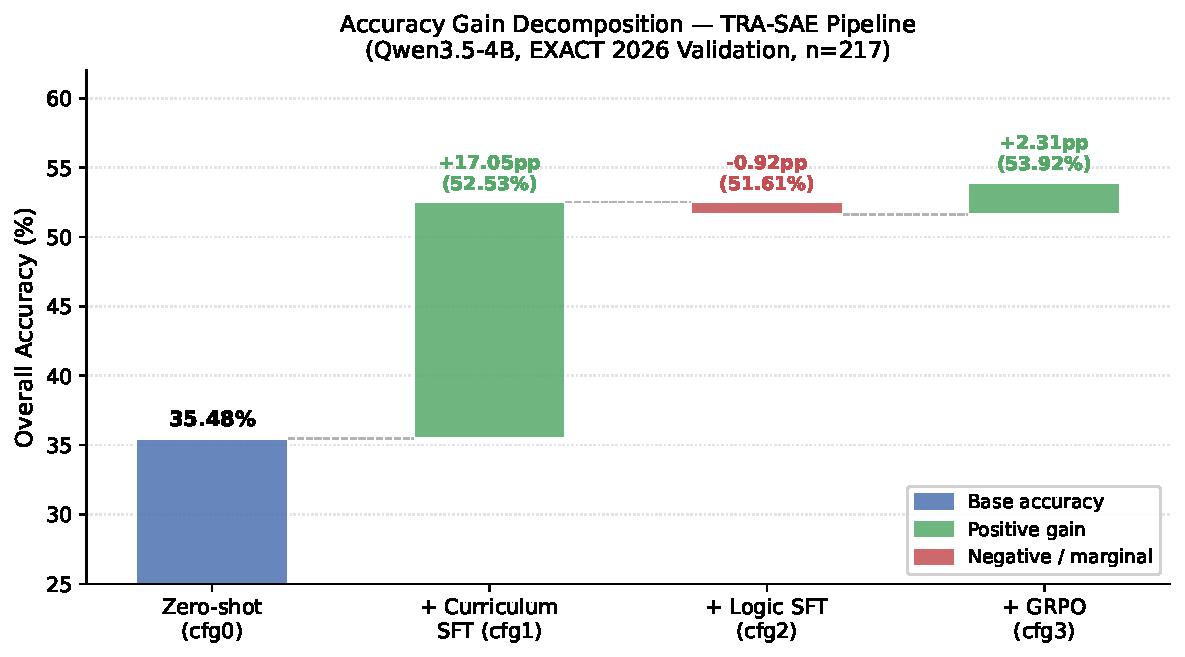
\includegraphics[width=0.90\columnwidth]{fig_decomposition}
  \caption{Accuracy gain decomposition across the \modelname{} pipeline.
           Each bar shows the change relative to the previous stage.
           Curriculum SFT (cfg0 $\to$ cfg1) dominates with $+17.05$~pp;
           GRPO (cfg2 $\to$ cfg3) adds $+2.31$~pp.}
  \label{fig:decomposition}
\end{figure}

Figure~\ref{fig:decomposition} visualises the gain decomposition across
the four pipeline stages.
The dominance of curriculum SFT is visually unambiguous.

\textbf{Finding 1: Curriculum SFT provides the largest gain.}
cfg1 (SFT Phase 1) adds $+17.05$~pp over cfg0 zero-shot, while
GRPO further adds $+1.39$~pp. Curriculum SFT is therefore the dominant
training signal at this model scale and data budget.

\textbf{Finding 2: Auxiliary reward shaping is budget-sensitive.}
At a short 150-step budget, correctness-only (R4) achieves the highest
accuracy (41.47\%), outperforming the full reward mixture R1 (39.63\%).
Removing the unit-consistency term (R2) yields only $-0.46$~pp.
These results indicate that auxiliary format and unit-consistency rewards
do not pay off within 150 steps; we hypothesise that longer training is
required for shaping rewards to provide net benefit, though this could
not be verified within our compute budget.

\textbf{Finding 3: Self-consistency and Dual-LoRA routing do not help at 4B.}
cfg5 (SC + Dual-LoRA) is $3.23$~pp \emph{worse} than cfg3.
We attribute this to the Dual-LoRA switch causing interference on
borderline-domain questions, and SC adding noise rather than consensus
at this model capacity.

\textbf{Finding 4: Logic remains a bottleneck.}
Logic accuracy peaks at $30.26\%$ (cfg4), compared to $67.38\%$ physics,
suggesting that formal logical inference requires capabilities beyond
standard SFT/GRPO at the 4B scale.

% ============================================================
\section{Discussion}
\label{sec:discussion}
% ============================================================

\subsection{When Does Self-Consistency Fail?}

Self-consistency is effective when a model's errors are random across
independent samples~\cite{Wang2023sc}. At 4B scale, however, errors are
often \emph{systematic}: the model consistently applies the wrong formula
or misidentifies the quantifier, producing identical wrong answers across all
$N=5$ samples. Majority voting then reinforces the systematic error.

Table~\ref{tab:sc_failures} shows three representative failure patterns
identified from cfg5 predictions in \texttt{logs/phase4\_results.jsonl}.

\begin{table}[t]
  \centering
  \caption{Representative SC failure patterns from cfg5 ($N=5$ samples).
           In each case, all 5 samples agree on the same wrong answer.}
  \label{tab:sc_failures}
  \begin{tabular}{p{2.5cm}p{5.5cm}p{2.5cm}}
    \toprule
    \textbf{Pattern} & \textbf{Example} & \textbf{SC outcome} \\
    \midrule
    Wrong quantifier application
      & Premises imply ``Unknown''; model applies modus ponens regardless,
        answers ``A'' or ``Yes'' on all 5 samples
      & Majority reinforces wrong answer \\
    \addlinespace
    Answer-format mismatch
      & Ground truth is ``Do not change'' (qualitative); model computes
        $Q = CV = 100\,\mu\text{C}$ in all 5 samples
      & 5/5 agree on wrong value \\
    \addlinespace
    Free-text extraction failure
      & Model embeds answer in prose rather than
        $\langle$\texttt{answer}$\rangle$ tag on all 5 samples;
        extractor scores all as wrong
      & 5/5 wrong; SC cannot compensate \\
    \bottomrule
  \end{tabular}
\end{table}

These failure patterns explain why cfg5 (50.69\%) underperforms cfg3
(53.92\%) despite using five times the inference compute.
SC is most valuable when errors are sampler-noise-driven; our error
taxonomy (Table~\ref{tab:errors}) shows that 55.3\% of failures are
systematic E4 (logical fallacy) errors, precisely the regime where SC
provides no benefit.


\subsection{Router Limitations}

TF-IDF classification achieves $\sim$90\% accuracy on clean physics/logic
labels, but the 10\% border-zone questions (e.g., physics problems framed
as logical conditionals) are disproportionately difficult and get routed to
the wrong adapter. A neural routing layer trained end-to-end may help.

\subsection{Limitations}

\begin{itemize}
  \item \emph{Small, single-domain validation set.}
        With 217 samples, CIs span $\pm$7~pp and differences below
        $\approx$5~pp cannot be declared statistically significant.
        All conclusions should be interpreted within this uncertainty,
        especially the GRPO-over-SFT margin ($+1.39$~pp, $p=0.50$).

  \item \emph{Reward ablation conclusions are budget-conditional.}
        The finding that correctness-only (R4) outperforms the full
        reward mixture (R1) holds at a 150-step budget.
        The relative ordering may reverse at longer training horizons,
        which we could not verify due to compute constraints.

  \item \emph{Baseline numbers are extraction-sensitive.}
        Several 7B baselines achieve low scores primarily due to XML
        format non-compliance; their true reasoning capability is
        likely higher under tailored prompting.
        We report them as-is for reproducibility but caution against
        treating them as ceiling comparisons.

  \item \emph{Non-neural domain router.}
        The TF-IDF + logistic-regression router achieves $\approx$90\%
        classification accuracy but systematically mis-routes physics
        problems framed as logical conditionals.
        A neural router trained end-to-end is likely to reduce
        border-zone errors.

  \item \emph{Single-benchmark evaluation.}
        All experiments use the \dataset{} training and validation splits.
        Generalisation to broader scientific benchmarks
        (SciBench~\cite{Wang2024scibench}, GPQA~\cite{Rein2023}) is
        untested; curriculum composition would need adaptation.

  \item \emph{Logic gap requires neuro-symbolic approaches.}
        The 38.4-pp physics/logic accuracy gap, combined with the
        55.3\% logical-fallacy error rate, indicates that standard SFT
        and GRPO are insufficient for formal symbolic logic at 4B scale.
        Integrating Z3-guided reward signals or step-level supervision
        is the most promising direction for closing this gap.
\end{itemize}

% ============================================================
\section{Conclusion}
\label{sec:conclusion}
% ============================================================

We presented \modelname{}, a low-cost curriculum training pipeline for
mixed-domain scientific reasoning that combines curriculum SFT, GRPO with
lightweight reward shaping, and an optional Dual-LoRA routing agent.
Our best configuration achieves $53.92\%$ overall accuracy on the
\dataset{} validation set, a $+18.44$~pp improvement over the
\basemodelname{} zero-shot baseline, using only a 4B-parameter open-source
model and under \$64 of total compute.

The primary empirical finding is that \emph{curriculum SFT is the dominant
training signal}: the transition from zero-shot to SFT contributes
$+17.05$~pp, while subsequent GRPO training adds a smaller $+1.39$~pp.
Reward ablations further show that correctness-only training is more
sample-efficient at short budgets, and auxiliary unit-consistency /
format rewards require longer training horizons to provide net benefit.
A significant set of negative results---self-consistency voting and
Dual-LoRA routing both degrade performance---provides actionable guidance
on where compute is best not spent at 4B scale.
Finally, a structured error taxonomy reveals that formal-logic errors
dominate failures ($55.3\%$), pointing to neuro-symbolic or
solver-augmented reasoning as the most promising direction for improvement.

Future work will explore (i)~scaling to 7B/14B checkpoints,
(ii)~process-level reward via step-annotated data,
(iii)~cross-dataset evaluation on SciBench and GPQA, and
(iv)~integrating Z3-guided training signals to address the logic gap.

% ── Acknowledgements ───────────────────────────────────────
\section*{Acknowledgements}
\todo{Add acknowledgements if applicable.}

% ── References ─────────────────────────────────────────────
\bibliographystyle{IEEEtran}
\bibliography{references}

\EOD
\end{document}
